\section{Neural Networks}\label{sec:ch2:cnns}
\subsection{The Neuron and Single Layer Neural Networks}

\begin{figure}
  \centering
  \pagestyle{empty}

\def\layersep{2.5cm}

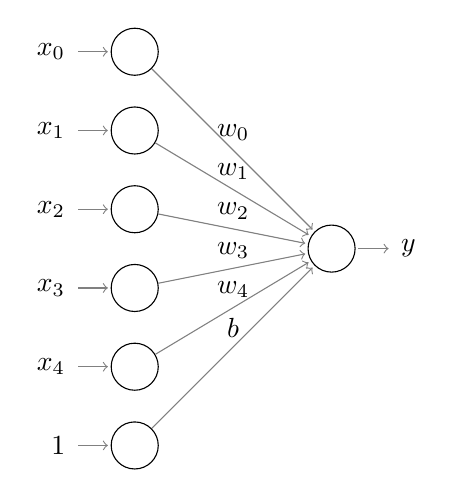
\begin{tikzpicture}[shorten >=1pt,->,draw=black!50, node distance=\layersep]
    \tikzstyle{every pin edge}=[<-,shorten <=1pt]
    \tikzstyle{neuron}=[circle,draw=black,minimum size=17pt,inner sep=0pt]
    \tikzstyle{input neuron}=[neuron];
    \tikzstyle{output neuron}=[neuron, fill=red!50];
    \tikzstyle{hidden neuron}=[neuron];
    \tikzstyle{annot} = [text width=4em, text centered]

    % Draw the input layer nodes
    \foreach \name / \y in {0,...,4}
    % This is the same as writing \foreach \name / \y in {1/1,2/2,3/3,4/4}
        \node[input neuron,pin=left:$x_\y$] (I-\name) at (0,-\y) {};
    \node[input neuron,pin=left:1] (I-5) at (0,-5) {};

    % Draw the output layer node
    \node[hidden neuron,pin={[pin edge={->}]right:$y$}] (O) at (\layersep, -2.5) {};

    % Connect every node in the input layer with every node in the
    % hidden layer.
    % \foreach \source in {1,...,5}
        % \draw(I-\source) edge (O) node[above, midway] {$w_\source$};
    \foreach \source in {0,...,4}
        \draw[->] (I-\source) -- (O) node[above,midway] {$w_\source$};
    \draw[->] (I-5) -- (O) node[above,midway] {$b$};

    % Annotate the layers
    % \node[annot,above of=I-1, node distance=1cm] (il) {Input Layer};
    % \node[annot,right of=hl] {Output layer};
\end{tikzpicture}
% End of code

  \mycaption{A single neuron}{The neuron is composed of inputs $x_i$, weights
    $w_i$ (and a bias term), as well as an activation function. Typical activation
    functions include the sigmoid function, tanh function and the ReLU}
  \label{fig:ch2:singlelayer}
\end{figure}

The neuron, shown in \autoref{fig:ch2:singlelayer} is the core building block of
Neural Networks. It takes the dot product between an input vector $\vec{x} \in
\reals[D]$ and a weight vector $\vec{w}$, before applying a chosen nonlinearity,
$g$. I.e.
%
\begin{equation}
  y = g(\langle\vec{x}, \vec{w}\rangle) = g\left(\sum_{i=0}^{D} x_i w_i \right) 
\end{equation}
%
where we have used the shorthand $b=w_0$ and $x_0 = 1$. Also note that we will
use the neural network common practice of calling the \emph{weights} $w$,
compared to the parameters $\theta$ we have been discussing thus far.

Typical nonlinear functions $g$ are the sigmoid function (already presented in 
\eqref{eq:ch2:sigmoid}), but also common are the tanh and ReLU functions:
\begin{eqnarray}
  \F{tanh}(x) &=& \frac{e^{x} - e^{-x}}{e^{x} + e^{-x}} \label{eq:ch2:tanh}\\
  \F{ReLU}(x) &=& \max (x, 0) \label{eq:ch2:relu}
\end{eqnarray}

See \autoref{fig:ch2:nonlinearities} for plots of these. The original Rosenblatt
perceptron \cite{rosenblatt_perceptron:_1958} used the Heaviside function
$\F{H}(x) = \mathbb{I}(x > 0)$. % The sigmoid nonlinearity
% naturally arises when we want to do classification with class labels $\{0,1\}$,
% as does the tanh function for classification with class labels $\{-1, 1\}$. The
% ReLU however is used more often in deeper architectures
% \cite{nair_rectified_2010}.

Note that if $\langle\vec{w}, \vec{w}\rangle = 1$ then $\langle\vec{x},
\vec{w}\rangle$ is the distance from the point $\vec{x}$ to the hyperplane with
normal $\vec{w}$. With general $\vec{w}$ this can be thought of as a scaled
distance. Thus, the weight vector $\vec{w}$ defines a hyperplane in $\reals[D]$
which splits the space into two. The choice of nonlinearity then affects how
points on each side of the plane are treated. For a sigmoid, points far below
the plane get mapped to 0 and points far above the plane get mapped to 1 (with
points near the plane having a value of 0.5). For tanh nonlinearities, these
points get mapped to -1 and 1. For ReLU nonlinearities, every point below the
plane ($\langle\vec{x}, \vec{w}\rangle < 0$) gets mapped to zero and every point
above the plane keeps its inner product value. 

Nearly all modern neural networks use the ReLU nonlinearity and it has
been credited with being a key reason for the recent surge in deep learning
success \cite{glorot_deep_2011, nair_rectified_2010}. In particular:
\begin{enumerate}
\item It is less sensitive to initial conditions as the gradients that
  backpropagate through it will be large even if $x$ is large. A common
  observation of sigmoid and tanh non-linearities was that their learning would
  be slow for quite some time until the neurons came out of saturation, and then
  their accuracy would increase rapidly before levelling out again at
  a minimum~\citep{glorot_understanding_2010}. The ReLU, on the other hand, has
  constant gradient.
\item It promotes sparsity in outputs, by setting them to a hard 0. Studies
  on brain energy expenditure suggest that neurons encode information in
  a sparse manner. \citet{lennie_cost_2003} estimates the percentage of
  neurons active at the same time to be between 1 and 4\%. Sigmoid and tanh
  functions will typically have \emph{all} neurons firing, while 
  the ReLU can allow neurons to fully turn off.
\end{enumerate}

\begin{figure}
    \qquad
    \section{Wavelet-Based Nonlinearities}\label{sec:ch6:nonlinearities}
Returning to the goals from \autoref{sec:ch6:learning}, the experiments from the
previous section have shown that while it is possible to use a wavelet gain
layer ($G$) in place of a convolutional layer ($H$), this may come with a small
performance penalty. Ignoring this effect for the moment, in this section, we
continue with our investigations into learning in the wavelet domain. In
particular, is it possible to replace a pixel domain nonlinearity $\sigma$ with
a wavelet-based one $\sigma_w$?

But what sensible nonlinearity should be used? Two particular options are good initial
candidates:
\begin{enumerate}
  \item The ReLU: this is a mainstay of most modern neural networks and has
    proved invaluable in the pixel domain. Its pseudo-nonlinearity
    ($\F{ReLU}(Ax) = A\F{ReLU}(x)$) makes learning less dependent on signal
    amplitudes. Perhaps its sparsifying
    properties will work well on wavelet coefficients too. 
  \item Thresholding: a technique commonly applied to wavelet
    coefficients for denoising and compression. Many proponents of compressed
    sensing and dictionary learning even like to compare soft thresholding to a
    two-sided ReLU \cite{papyan_theoretical_2018, papyan_convolutional_2017-1}.
\end{enumerate}

In this section, we will look at both and see if they improve the gain
layer. If they do, it would the be possible to connect multiple layers in the
wavelet domain, avoiding the necessity to do inverse wavelet transforms after
learning.

\subsection{ReLUs in the Wavelet Domain}
Applying the ReLU to the real lowpass coefficients is not difficult, but it does
not generalize so easily to complex coefficients. The simplest option is to apply
it independently to the real and imaginary coefficients, effectively only
selecting one quadrant of the complex plane:
\begin{align}
  u_{lp} &= \F{max}(0,\ v_{lp}) \\
  u_{j} &= \F{max}(0,\ \real{v_{j}}) + j\F{max}(0,\ \imag{v_j}) \label{eq:ch6:relu_bp}
\end{align}

Another option is to apply it to the magnitude of the bandpass coefficients. Of
course, these are all strictly positive so the ReLU on its own would not do
anything. However, they can be arbitrarily scaled and shifted by using a batch
normalization layer. Then the magnitude could shift to (invalid) negative
values, which can then be rectified by the ReLU.

Dropping the scale subscript $j$ for clarity (we need it for the square root of 
negative 1), let a bandpass coefficient at a given scale be
$v = r_v e^{j\theta_v}$ and define
$\mu_r = \mathbb{E}[r_v]$ and $\sigma_r^2 = \mathbb{E}[(r_v-\mu_r)^2]$, then
applying batch-normalization and the ReLU to the magnitude of $v_j$ means we
get:
\begin{align}
  r_u &= \F{ReLU}(BN(r_v)) = \max(0,\ \gamma \frac{r_v-\mu_r}{\sigma_r} + \beta) \label{eq:ch6:magrelu_bp} \\
  u &= r_u e^{j\theta_v} \label{eq:ch6:magrelu_bp2}
\end{align}
This also works equivalently on the lowpass coefficients, although $v_{lp}$ can
be negative unlike $r_v$:
\begin{equation}
  u_{lp} = \F{ReLU}(BN(v_{lp})) = \max(0, \gamma' \frac{v_{lp} - \mu_{lp}}{\sigma_{lp}} + \beta') \label{eq:ch6:bnrelu_lp}
\end{equation}
%
\subsection{Thresholding}
For $t \in \reals$ and $z = re^{j\theta} \in \complexes$ the pointwise hard thresholding is:
\begin{align}
  \mathcal{H}(z, t) &= \left\{ \begin{array}{ll}
    z & r \geq t \\
    0 & r < t\\
  \end{array} \right. \\
  &= \indic(r > t) z
\end{align}
and the pointwise soft thresholding is:
\begin{align}
  \mathcal{S}(z, t) &= \left\{ \begin{array}{ll}
    (r-t)e^{j\theta} & r \geq t \\
    0 & r < t\\
  \end{array} \right. \\
  &= \max(0, r - t)e^{j\theta} \label{eq:ch6:relu_st}
\end{align}
Note that \eqref{eq:ch6:relu_st} is very similar to \eqref{eq:ch6:magrelu_bp} and \eqref{eq:ch6:magrelu_bp2}.
We can rewrite \eqref{eq:ch6:magrelu_bp} by taking the strictly positive terms
$\gamma$, $\sigma$ outside of the $\max$ operator:
\begin{align}
  r_u &= \max(0, \gamma \frac{r_v-\mu_r}{\sigma_r} + \beta) \\
      &= \frac{\gamma}{\sigma_r}\max\left(0, r_v - \left(\mu_r - \frac{\sigma_r\beta}{\gamma}\right)\right) \label{eq:ch6:bnrelu_soft}
\end{align}
then if $t' = \mu_v - \frac{\sigma_r\beta}{\gamma} > 0$, \textbf{doing batch
normalization followed by a ReLU on the magnitude of the complex coefficients is the
same as soft shrinkage with threshold $t'$, scaled by a factor
$\frac{\gamma}{\sigma_r}$}.

The same analogy does not apply to the lowpass
coefficients, as $v_{lp}$ is not strictly positive.

While soft thresholding is similar to batch normalizations and ReLUs, we would also like
to test how well it performs as a sparsity-inducing wavelet nonlinearity.
To do this, we can:
\begin{itemize}
  \item Learn the threshold $t$
  \item Adapt $t$ as a function of the distribution of activations to achieve a desired sparsity level.
\end{itemize}
In early experiments, we found that trying to set
desired sparsity levels by tracking the standard deviation of the statistics
and setting a threshold as a function of it performed very poorly (causing a
drop in top-1 accuracy of at least 10\%).
Instead, we choose to learn a threshold $t$. We make this an unconstrained
optimization problem by changing \eqref{eq:ch6:relu_st} to:
\begin{equation}
  \mathcal{S}(v, t) = \max(0, r-|t|)e^{j\theta}  \label{eq:ch6:relu_st2}
\end{equation}

Learning a threshold is only possible for soft thresholding, as $\dydx{L}{t}$ is
not defined for hard thresholding. Like batch normalization, we learn
independent thresholds $t$ for each channel.

    \quad
    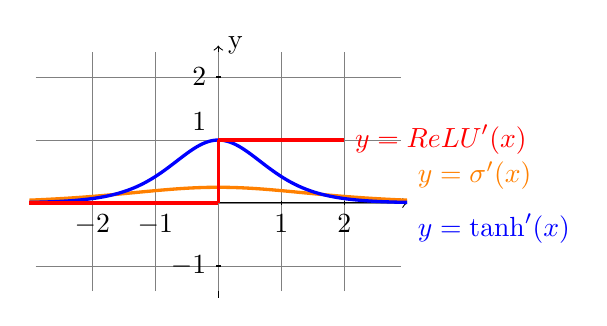
\begin{tikzpicture}[scale=0.8]
  % Draw axes
  \draw[->] (-3,0) -- (3,0);
  \draw[->] (0,-1.5) -- (0,2.5) node[right] {y};

  % Draw gridlines
  \draw[step=1cm,gray,very thin] (-2.9,-1.4) grid (2.9, 2.4);

  \foreach \x in {-2,-1,1,2}
    \draw (\x cm,1pt) -- (\x cm,-1pt) node[anchor=north] {$\x$};
  \foreach \y in {-1,  2}
    \draw (1pt, \y cm) -- (-1pt, \y cm) node[anchor=east] {$\y$};
  \draw (1pt, 1 cm) -- (-1pt, 1 cm) node[anchor=south east] {$1$};

  % Draw sigmoid
  \draw[orange, very thick, domain=-3:3, samples=200] plot (\x, {(exp(-\x)/(1+exp(-\x))^2})
    node[above right] {$y=\sigma'(x)$};

  % Draw Tanh
  \draw[blue, very thick, domain=-3:3, samples=200] plot (\x, {1 - ((exp(\x)-exp(-\x))/(exp(\x)+exp(-\x)))^2})
    node[below right] {$y=\tanh'(x)$};

  % Draw ReLU
  \draw[red, very thick, domain=-3:0, samples=5] plot (\x, {0});
  \draw[red, very thick] (0, 0) -- (0, 1);
  \draw[red, very thick, domain=0:2, samples=5] plot (\x, {1}) node[right]
    {$y=\F{ReLU}'(x)$};

\end{tikzpicture}


  \centering
  \mycaption{Common Neural Network nonlinearities and their gradients}{The sigmoid, tanh and ReLU
  nonlinearities are commonly used activation functions for neurons. Note the
  different properties. In particular, the tanh and sigmoid have the nice
  property of being smooth but can have saturation when the input is either
  largely positive or largely negative, causing little gradient to flow back
  through it. The ReLU does not suffer from this problem, and has the additional
  nice property of setting values to exactly 0, making a sparser output
  activation.}
  \label{fig:ch2:nonlinearities}
\end{figure}

\subsection{Multilayer Perceptrons}
As mentioned in the previous section, a single neuron can be thought of as a
separating hyperplane with an activation that maps the two halves of the space
to different values. Such a linear separator is limited, and famously cannot
solve the XOR problem \cite{minsky_perceptrons:_1988}. Fortunately, adding a
single hidden layer like the one shown in \autoref{fig:ch2:hidden} can change
this, and it is provable that with an infinitely wide hidden layer, a neural
network can approximate any function \cite{hornik_multilayer_1989,
cybenko_approximation_1989}. 

The forward pass of such a network with one hidden layer of $H$ units is:
%
\begin{eqnarray}
  h_i & = & g\left(\sum_{j=0}^{D} x_j w_{ij}^{(1)}\right) \\
  y & = & \sum_{k=0}^{H} h_k w^{(2)}_{k}
\end{eqnarray}
%
where $w^{(l)}$ denotes the weights for the $l$-th layer, of which
\autoref{fig:ch2:hidden} has 2. Note that these individual layers are often
called \emph{fully connected} as each node in the previous layer affects every
node in the next.

If we were to expand this network to have $L$ such fully connected layers, we
could rewrite the action of each layer in a recursive fashion:
%
\begin{eqnarray}
  Y^{(l+1)} &=& W^{(l+1)}X^{(l)} \\
  X^{(l+1)} &=& g\left(Y^{(l+1)}\right) 
\end{eqnarray}
where $W$ is now a weight matrix, acting on the vector of previous layer's
outputs $X^{(l)}$. As we are now considering every layer an input to the next
stage, we have removed the $h$ notation, and added the superscript $(l)$ to
define the depth. $X^{(0)}$ is the network input and $Y^{(L)}$ is the network
output. Let us say that the output has $C$ nodes, and a hidden layer $X^{(l)}$
has $C_l$ nodes.

\begin{figure}[t]
  \centering
  % MLP
\begin{tikzpicture}[scale=1]
    \def\nodedist{35pt}
    \def\layerdist{80pt}
    \def\pindist{20pt}
    
    \tikzstyle{every pin edge}=[signal]
    \tikzstyle{annot} = [text width=4em, text centered]
    
    \foreach \y in {1,...,3}
        \node[inputnode, pin={[pin edge={latex-}, pin distance=\pindist]left:Input \y}] 
            (I\y) at (0,-\y*\nodedist) {$x_\y$};  
    
    \foreach \y in {1,...,4}
        \node[hiddennode] 
            (H\y) at ($(\layerdist,-\y*\nodedist) +(0, 0.5*\nodedist)$) {$h_\y$};
    
    \foreach \y in {1,...,1}
        \node[outputnode, pin={[pin edge={-latex}, pin distance=\pindist]right:Output \y}]
            (O\y) at ($(I2) + (2*\layerdist, 0)$) {$y_\y$};
    
    \foreach \dest in {1,...,4}
        \foreach \source in {1,...,3}
            \draw[signal] (I\source) -- (H\dest);
    
    \foreach \dest in {1,...,1}
        \foreach \source in {1,...,4}
            \draw[signal] (H\source) edge (O\dest);
    
    \node[annot, above=4pt of H1] (hl) {Hidden layer};
    \node[annot] at (I1 |- hl) {Input layer};
    \node[annot] at (O1 |- hl) {Output layer};
\end{tikzpicture}

  \mycaption{Multi-layer perceptron}{Expanding the single neuron from 
  \autoref{fig:ch2:singlelayer} to a network of neurons. The internal
  representation units are often referred to as the \emph{hidden layer} as they
  are an intermediary between the input and output.}
  \label{fig:ch2:hidden}
\end{figure}

\subsection{Backpropagation}
It is important to truly understand backpropagation when designing neural
networks, so we describe the core concepts now for a neural network with
$L$ layers.

The delta rule, initially designed for networks with no hidden layers 
\cite{widrow_neurocomputing:_1988}, was expanded to what we now consider
\emph{backpropagation} in \cite{rumelhart_parallel_1986}. While backpropagation
is conceptually just the application of the chain rule, Rumelhart, Hinton, and
Williams successfully updated the delta rule to networks with hidden layers,
laying a key foundational step for deeper networks. 

With a deep network, calculating $\dydx{J}{w}$ may not seem
particularly obvious if $w$ is a weight in one of the earlier layers. We need
to define a rule for updating the weights in all $L$ layers of the network,
$W^{(1)}, W^{(2)}, \ldots W^{(L)}$ however, only the final set $W^{(L)}$ are
connected to the objective function $J$. 

\subsubsection{Regression Loss}
Let us start with writing down the derivative of $J$ with respect to the network
output $Y^{(L)}$ using the regression objective function \eqref{eq:ch2:mle_reg}. 
As we now have two superscripts,
one for the sample number and one for the layer number, we combine them into a
tuple of superscripts. 
\begin{eqnarray}
  \dydx{J}{Y^{(L)}} &= & \dydx{}{Y^{(L)}} \left( \frac{1}{N}\sum_{n=1}^{N_b}\frac{1}{2} \left(y^{(n)} - Y^{(L, n)}\right)^2\right) \\
                    &=& \frac{1}{N}\sum_{n=1}^{N_b} \left(Y^{(L, n)} - y^{(n)} \right) \\
                    &=& e \in \reals \label{eq:ch2:reg_b1}
\end{eqnarray}
where we have used the fact that for the regression case, $y^{(n)}, Y^{(L,n)}
\in \reals$. 

\subsubsection{Classification Loss}
For the classification case \eqref{eq:ch2:mle_class}, let us keep the output of
the network $Y^{(L,n)} \in \reals[C]$ and define an intermediate value $\hat{y}$ the
softmax applied to this vector $\hat{y}^{(n)}_c = \sigma_c\left(Y^{(L, n)}\right)$.
Note that this is a vector valued function going from $\reals[C] \rightarrow
\reals[C]$ so has a jacobian matrix $S_{ij} = \dydx{\hat{y}_i}{Y^{(L)}_j}$ with
values:
\begin{equation}
  S_{ij} = \begin{cases}
    \sigma_i (1-\sigma_j) & \text{if $i=j$}\\
    -\sigma_i \sigma_j & \text{if $i\neq j$}\\
  \end{cases}
\end{equation}

Now, let us return to \eqref{eq:ch2:mle_class} and find the derivative of the
objective function to this intermediate value $\hat{y}$:
\begin{eqnarray}
  \dydx{J}{\hat{y}} &= & \dydx{}{\hat{y}} \left( \frac{1}{N}\sum_{n=1}^{N_b} \sum_{c=1}^C 
  y^{(n)}_c \log \hat{y}^{(n)}_c \right) \\
  &=& \frac{1}{N}\sum_{n=1}^{N_b} \sum_{c=1}^C \frac{y^{(n)}_c}{\hat{y}^{(n)}_c} \\
  &=& d \in \reals[C] \label{eq:ch2:class_b1}
\end{eqnarray}
Note that unlike \eqref{eq:ch2:reg_b1}, this derivative is vector valued. To
find $\dydx{J}{Y^{(L)}}$ we use the chain rule. It is easier to find the
partial derivative with respect to one node in the output first, and then expand
from here. I.e.:

\begin{eqnarray}
  \dydx{J}{Y^{(L)}_j} &=& \sum_{i=1}^C \dydx{J}{\hat{y}_i}\dydx{\hat{y}_i}{Y^{(L)}_j} \\
                      &=& S_i^T d
\end{eqnarray}
where $S_i$ is the $i$th column of the jacobian matrix $S$. It becomes clear now
that to get the entire vector derivative for all nodes in $Y^{(L)}$, we must
multiply the transpose of the jacobian matrix with the error term from
\eqref{eq:ch2:class_b1}:
\begin{equation}
  \dydx{J}{Y^{(L)}} = S^T d
\end{equation}

\subsubsection{Final Layer Weight Gradient} \label{sec:ch2:weight}
Let us continue by assuming $\dydx{J}{Y^{(L)}}$ is vector valued as was the case
with classification. For regression, it is easy to set $C=1$ in the following to
get the necessary results. Additionally for clarity, we will drop the layer
superscript in the intermediate calculations.

We call the gradient for the final layer weights the \emph{update} gradient. 
It can be computed by the chain rule again:
\begin{eqnarray}
  \dydx{J}{W_{ij}} &=& \dydx{J}{Y_i} \dydx{Y_i}{W_{ij}} + 2\lambda W_{ij} \\
  &=& \dydx{J}{Y_i} X_j + 2\lambda W_{ij}
\end{eqnarray}
where the second term in the above two equations comes from the regularization
loss that is added to the objective. The gradient of the entire weight matrix is 
then:
\begin{eqnarray}
  \dydx{J}{W^{(L)}} &=& \dydx{J}{\hat{y}} X^T +2\lambda W \\
   &=& S^T d \left(X^{(L-1)}\right)^T + 2\lambda W^{(L)} \in \reals[C \x C_{L-1}]
\end{eqnarray}

\subsubsection{Final Layer Passthrough Gradient} \label{sec:ch2:passthrough}
Additionally, we want to find the \emph{passthrough} gradients of the final
layer $\dydx{J}{X^{(L-1)}}$. In a similar fashion, we first find the gradient
with respect to individual elements in $X^{(L-1)}$ before generalizing to the
entire vector:
\begin{eqnarray}
  \dydx{J}{X_i} &=& \sum_{j=1}^{C} \dydx{J}{Y_j} \dydx{Y_j}{X_i} \\
                &=& \sum_{j=1}^{C} \dydx{J}{Y_j} W_{j,i} \\
                &=& W_{i}^T\dydx{J}{Y} \\
\end{eqnarray}
where $W_i$ is the $i$th column of $W$. Thus
\begin{eqnarray}
  \dydx{J}{X^{(L-1)}} &=& \left(W^{(L)}\right)^T \dydx{J}{Y^{(L)}} \\
                      &=& \left( W^{(L)} \right)^T S^T d
\end{eqnarray}
This passthrough gradient then can be used to update the next layer's weights by
repeating \autoref{sec:ch2:weight} and \autoref{sec:ch2:passthrough}.

\subsubsection{General Layer Update}
The easiest way to handle this flow of gradients, and the basis for most
automatic differentiation packages, is the block definition shown in
\autoref{fig:ch2:block_form}. For all neural network components (even if they do
not have weights), the operationg must not only be able to calculate the forward 
pass $y=f(x, w)$ given weights $w$ and inputs $x$, but also calculate the
\emph{update} and \emph{passthrough} gradients $\dydx{J}{w}, \dydx{J}{x}$ given
an input gradient $\dydx{J}{y}$. The input gradient will have the same shape as
$y$ as will the update and passthrough gradients match the shape of $w$ and $x$.
This way, gradients for the entire network cam be computed in an iterative
fashion starting at the loss function and moving backwards.

\begin{figure}
  \centering
  \begin{tikzpicture}[every node/.style={node font=\large}]
\definecolor{mycolor}{RGB}{252,247,189};
\pgfmathsetmacro{\EDGE}{.5}
\node [fill=mycolor, draw, minimum width=3cm, minimum height=2cm] (block) at (1,1) {$y=f(x,w)$};
\coordinate[right=\EDGE of block.south west] (xin);
\coordinate[left=\EDGE of block.south east] (dxin);
\coordinate[below=\EDGE of block.north west] (win);
\coordinate[above=\EDGE of block.south west] (dwin);
\coordinate[right=\EDGE of block.north west] (yin);
\coordinate[left=\EDGE of block.north east] (dyin);
\draw[<-] (xin) -- +(0,-1) node[below] {$x$};
\draw[->] (dxin) -- ++(0,-1) node[below] {$\dydx{\logloss}{x}$};
\draw[<-] (win) -- ++(-1,0) node[left] {$w$};
\draw[->] (dwin) -- ++(-1,0) node[left] {$\dydx{\logloss}{w}$};
\draw[->] (yin) -- ++(0,1) node[above] {$y$};
\draw[<-] (dyin) -- ++(0,1) node[above] {$\dydx{\logloss}{y}$};
\end{tikzpicture}

  \mycaption{General block form for autograd}{All neural network functions
  need to be able to calculate the forward pass $y=f(x,w)$ as well as the 
  update and passthrough gradients $\dydx{J}{w}, \dydx{J}{x}$. Backpropagation
  is then easily done by allowing data to flow backwards through these blocks
  from the loss.}
  \label{fig:ch2:block_form}
\end{figure}

\subsection{Extending to multiple layers and different block types}

\subsubsection{Convolutional Layers}
  The image/layer of features is convolved by a set of filters.
  The filters are typically small, ranging from $3\x 3$ in ResNet and VGG
  to $11\x 11$ in AlexNet. We have quoted only spatial size
  here, as the filters in a CNN are always \emph{fully connected in depth} ---
  i.e.,\ they will match the number of channels their input has.

  For an input $\bmu{x} \in \mathbb{R}^{H\x W\x D}$, and filters 
  $\bmu{f} \in \mathbb{R}^{H'\x W'  \x D \x D''}$ ($D''$ is the 
  number of filters), our output $\bmu{z} \in
  \mathbb{R}^{H''\x W'' \x D''}$ will be given by:
  \begin{equation}
    z[u_1, u_2, d''] = b[d''] + \sum_{i=-\frac{H'}{2}}^{\frac{H'}{2}-1}
                       \sum_{j=-\frac{W'}{2}}^{\frac{W'}{2}-1}  \sum_{k=0}^{D-1}  
                        f[i, j, k, d''] x[u_1-i, u_2-j, k]
  \end{equation}

\subsubsection{ReLUs}
  Activation functions, neurons, or non-linearities, are the core of a neural networks
  expressibility. Historically, they were sigmoid or tanh functions, but these
  have been replaced recently by the Rectified Linear Unit (ReLU), which has
  equation $g(x) = \max(0,x)$. A ReLU
  \begin{figure}
    \centering
      % \section{Wavelet-Based Nonlinearities}\label{sec:ch6:nonlinearities}
Returning to the goals from \autoref{sec:ch6:learning}, the experiments from the
previous section have shown that while it is possible to use a wavelet gain
layer ($G$) in place of a convolutional layer ($H$), this may come with a small
performance penalty. Ignoring this effect for the moment, in this section, we
continue with our investigations into learning in the wavelet domain. In
particular, is it possible to replace a pixel domain nonlinearity $\sigma$ with
a wavelet-based one $\sigma_w$?

But what sensible nonlinearity should be used? Two particular options are good initial
candidates:
\begin{enumerate}
  \item The ReLU: this is a mainstay of most modern neural networks and has
    proved invaluable in the pixel domain. Its pseudo-nonlinearity
    ($\F{ReLU}(Ax) = A\F{ReLU}(x)$) makes learning less dependent on signal
    amplitudes. Perhaps its sparsifying
    properties will work well on wavelet coefficients too. 
  \item Thresholding: a technique commonly applied to wavelet
    coefficients for denoising and compression. Many proponents of compressed
    sensing and dictionary learning even like to compare soft thresholding to a
    two-sided ReLU \cite{papyan_theoretical_2018, papyan_convolutional_2017-1}.
\end{enumerate}

In this section, we will look at both and see if they improve the gain
layer. If they do, it would the be possible to connect multiple layers in the
wavelet domain, avoiding the necessity to do inverse wavelet transforms after
learning.

\subsection{ReLUs in the Wavelet Domain}
Applying the ReLU to the real lowpass coefficients is not difficult, but it does
not generalize so easily to complex coefficients. The simplest option is to apply
it independently to the real and imaginary coefficients, effectively only
selecting one quadrant of the complex plane:
\begin{align}
  u_{lp} &= \F{max}(0,\ v_{lp}) \\
  u_{j} &= \F{max}(0,\ \real{v_{j}}) + j\F{max}(0,\ \imag{v_j}) \label{eq:ch6:relu_bp}
\end{align}

Another option is to apply it to the magnitude of the bandpass coefficients. Of
course, these are all strictly positive so the ReLU on its own would not do
anything. However, they can be arbitrarily scaled and shifted by using a batch
normalization layer. Then the magnitude could shift to (invalid) negative
values, which can then be rectified by the ReLU.

Dropping the scale subscript $j$ for clarity (we need it for the square root of 
negative 1), let a bandpass coefficient at a given scale be
$v = r_v e^{j\theta_v}$ and define
$\mu_r = \mathbb{E}[r_v]$ and $\sigma_r^2 = \mathbb{E}[(r_v-\mu_r)^2]$, then
applying batch-normalization and the ReLU to the magnitude of $v_j$ means we
get:
\begin{align}
  r_u &= \F{ReLU}(BN(r_v)) = \max(0,\ \gamma \frac{r_v-\mu_r}{\sigma_r} + \beta) \label{eq:ch6:magrelu_bp} \\
  u &= r_u e^{j\theta_v} \label{eq:ch6:magrelu_bp2}
\end{align}
This also works equivalently on the lowpass coefficients, although $v_{lp}$ can
be negative unlike $r_v$:
\begin{equation}
  u_{lp} = \F{ReLU}(BN(v_{lp})) = \max(0, \gamma' \frac{v_{lp} - \mu_{lp}}{\sigma_{lp}} + \beta') \label{eq:ch6:bnrelu_lp}
\end{equation}
%
\subsection{Thresholding}
For $t \in \reals$ and $z = re^{j\theta} \in \complexes$ the pointwise hard thresholding is:
\begin{align}
  \mathcal{H}(z, t) &= \left\{ \begin{array}{ll}
    z & r \geq t \\
    0 & r < t\\
  \end{array} \right. \\
  &= \indic(r > t) z
\end{align}
and the pointwise soft thresholding is:
\begin{align}
  \mathcal{S}(z, t) &= \left\{ \begin{array}{ll}
    (r-t)e^{j\theta} & r \geq t \\
    0 & r < t\\
  \end{array} \right. \\
  &= \max(0, r - t)e^{j\theta} \label{eq:ch6:relu_st}
\end{align}
Note that \eqref{eq:ch6:relu_st} is very similar to \eqref{eq:ch6:magrelu_bp} and \eqref{eq:ch6:magrelu_bp2}.
We can rewrite \eqref{eq:ch6:magrelu_bp} by taking the strictly positive terms
$\gamma$, $\sigma$ outside of the $\max$ operator:
\begin{align}
  r_u &= \max(0, \gamma \frac{r_v-\mu_r}{\sigma_r} + \beta) \\
      &= \frac{\gamma}{\sigma_r}\max\left(0, r_v - \left(\mu_r - \frac{\sigma_r\beta}{\gamma}\right)\right) \label{eq:ch6:bnrelu_soft}
\end{align}
then if $t' = \mu_v - \frac{\sigma_r\beta}{\gamma} > 0$, \textbf{doing batch
normalization followed by a ReLU on the magnitude of the complex coefficients is the
same as soft shrinkage with threshold $t'$, scaled by a factor
$\frac{\gamma}{\sigma_r}$}.

The same analogy does not apply to the lowpass
coefficients, as $v_{lp}$ is not strictly positive.

While soft thresholding is similar to batch normalizations and ReLUs, we would also like
to test how well it performs as a sparsity-inducing wavelet nonlinearity.
To do this, we can:
\begin{itemize}
  \item Learn the threshold $t$
  \item Adapt $t$ as a function of the distribution of activations to achieve a desired sparsity level.
\end{itemize}
In early experiments, we found that trying to set
desired sparsity levels by tracking the standard deviation of the statistics
and setting a threshold as a function of it performed very poorly (causing a
drop in top-1 accuracy of at least 10\%).
Instead, we choose to learn a threshold $t$. We make this an unconstrained
optimization problem by changing \eqref{eq:ch6:relu_st} to:
\begin{equation}
  \mathcal{S}(v, t) = \max(0, r-|t|)e^{j\theta}  \label{eq:ch6:relu_st2}
\end{equation}

Learning a threshold is only possible for soft thresholding, as $\dydx{L}{t}$ is
not defined for hard thresholding. Like batch normalization, we learn
independent thresholds $t$ for each channel.

      \caption[Differences in non-linearities]
              {Differences in non-linearities. Green --- the \emph{sigmoid} function, 
               Blue --- the \emph{tanh} function, and Red --- the \emph{ReLU}. The ReLU
               solves the problem of small gradients outside of the activation
               region (around $x=0$) as well as promoting sparsity.}\label{fig:ch2:nonlinearities}
  \end{figure}


\subsubsection{Pooling}
  Typically following a convolutional layer (but not strictly), activations are subsampled with
  max pooling. Pooling adds some invariance to shifts smaller than the pooling
  size at the cost of information loss. For this reason, small pooling is
  typically done often $2\x 2$ or $3\x 3$, and the invariance to larger shifts
  comes after multiple pooling (and convolutional) layers.
  
  While initial designs of max pooling would do it in non-overlapping regions, 
  AlexNet used $3\x 3$ pooling with stride 2 in their breakthrough design,
  quoting that it gave them an increase in accuracy of roughly $0.5\%$ and
  helped prevent their network from `overfitting'. More recent networks will
  typically employ either this or the original $2\x 2$ pooling with stride 2,
  see \autoref{fig:ch2:maxpool}. A review of pooling methods in
  \citep{mishkin_systematic_2016} found them both to perform equally well.
  
  \begin{figure}
    \centering
    % \subfloat[]{%
        % \input{tikz/maxpool.tex}\label{fig:maxpool_tight}
    % }
%    \newline
    \centering
    % \subfloat[]{%
        % \input{tikz/maxpool_overlap.tex}\label{fig:maxpool_overlap}
    % }
    \caption[Tight vs.\ overlapping pooling]
            {\subref{fig:ch2:maxpool_tight} Tight $2\x 2$ pooling with stride 2, vs
            \subref{fig:ch2:maxpool_overlap} overlapping $3\x 3$ pooling with
            stride 2. Overlapping pooling has the possibility of having one
            large activation copied to two positions in the reduced size
            feature map, which places more emphasis on the odd columns.}
    \label{fig:ch2:maxpool}
  \end{figure}

\subsubsection{Batch Normalization}
      Batch normalization proposed only very recently in
      \citep{ioffe_batch_2015} is a conceptually simpler technique. Despite
      that, it has become quite popular and has been found to be very useful.
      At its core, it is doing what standard normalization is doing, but also
      introduces two learnable parameters --- scale ($\gamma$) and offset
      ($\beta$). \eqref{eq:ch2:normalization} becomes:
      \begin{equation}
        \tilde{z}(u_1,u_2,d) = \gamma\frac{z-E[z]}{\sqrt{Var[z]}} + \beta 
				\label{eq:ch2:batch_normalization}
      \end{equation}
      These added parameters make it a \emph{renormalization} scheme, as instead of
      centring the data around zero with unit variance, it can be centred
      around an arbitrary value with arbitrary variance. S etting
      $\gamma = \sqrt{Var[z]}$ and $\beta = E[z]$, we would get the identity
      transform. Alternatively, setting $\gamma = 1$ and $\beta = 0$ (the
      initial conditions for these learnable parameters), we get standard
      normalization.
      
      The parameters $\gamma$ and $\beta$ are learned through backpropagation.
      As data are usually processed in batches, the gradients for $\gamma$ and
      $\beta$ are calculated per sample, and then averaged over the whole
      batch.

      From \autoref{eq:ch2:batch_normalization}, let us briefly use the hat
      notation to represent the standard normalized input:
      $\hat{z} = (z-E[z])/\sqrt{Var[z]}$, then:
      \begin{eqnarray}
        \tilde{z}^{(i)} & = & \gamma \hat{z}^{(i)} + \beta \nonumber\\
        \frac{\partial \mathcal{L}}{\partial \gamma}& =&
        \frac{1}{N}\sum_{i=1}^{N} \frac{\partial
        \mathcal{L}^{(i)}}{\partial \tilde{z}^{(i)}} \cdot \hat{z}^{(i)} \\
        \frac{\partial \mathcal{L}}{\partial \beta}& =&
        \frac{1}{N}\sum_{i=1}^{N} \frac{\partial
        \mathcal{L}^{(i)}}{\partial \tilde{z}^{(i)}} 
      \end{eqnarray}

      Batch normalization layers are typically placed \emph{between} convolutional layers
      and non-linearities. I.e.,\ if $Wu+b$ is the output of a convolutional
      layer, and $z=g(Wu+b)$ is the output of the non-linearity, then with the
      batch normalization step, we have:
      \begin{eqnarray}
        z &=& g(BN(Wu+b)) \nonumber\\
          &=& g(BN(Wu))
      \end{eqnarray}
      Where the bias term was ignored in the convolutional layer, as it can be
      fully merged with the `offset' parameter $\beta$.

      This has particular benefit of removing the sensitivity of our network to
      our initial weight scale, as for scalar $a$,
      \begin{equation}
        BN(Wu) = BN((aW)u)
      \end{equation}
      It is also particularly useful for backpropagation, as an increase in
      weights leads to \emph{smaller} gradients \citep{ioffe_batch_2015}, making
      the network far more resilient to the problems of vanishing and exploding
      gradients:
      \begin{eqnarray}
        \frac{\partial BN((aW)u)}{\partial u} & = & \frac{\partial
        BN(Wu)}{\partial u} \nonumber\\
        \frac{\partial BN((aW)u)}{\partial (aW)} & = & \frac{1}{a} \cdot \frac{\partial
        BN(Wu)}{\partial W} 
      \end{eqnarray}


\section{Relevant Architectures}

\subsection{LeNet}
\subsection{AlexNet}
\subsection{VGG}
\subsection{Residual Networks}
  The current state of the art design introduced a clever novel feature called
  a residual unit\citep{he_deep_2015,he_identity_2016}. The inspiration for their design came from the difficulties
  experienced in training deeper networks. Often, adding an extra layer would
  \emph{decrease} network performance. This is counter-intuitive as the deeper
  layers could simply learn the identity mapping, and achieve the same
  performance.

  To promote the chance of learning the identity mapping, they define
  a residual unit, shown in \autoref{fig:ch2:residual_unit}. If a desired mapping
  is denoted $\mathcal{H}(x)$, instead of trying to learn this, they instead
  learn $\mathcal{F}(x) = \mathcal{H}(x) - x$. 
  \begin{figure}
    \centering
    % 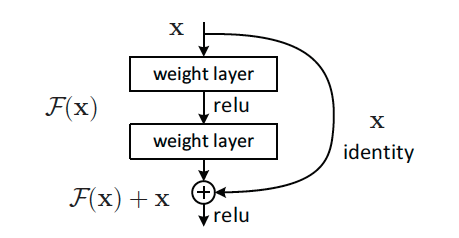
\includegraphics[width=0.5\textwidth]{images/residual_unit.png}
    \caption[The residual unit from ResNet]
          {A residual unit. The identity mapping is always present, and the
            network learns the difference from the identity mapping, $\mathcal{F}(x)$.
            Taken from \citep{he_deep_2015}.}
      \label{fig:ch2:residual_unit}
  \end{figure}


\subsection{old}
  Convolutional Neural Networks (CNNs) were initially introduced by \citet{lecun_backpropagation_1989} in
  \citep{lecun_backpropagation_1989}. Due to the difficulty of training and
  initializing them, they failed to be popular for more than two decades.  This
  changed in 2012, when advancements in pre-training with unsupervised networks
  \citep{bengio_greedy_2007}, the use of an improved non-linearity --- the Rectified Linear
  Unit, or ReLU, new regularization methods\citep{hinton_improving_2012}, and
  access to more powerful computers in graphics cards, or GPUs, allowed
  Krizhevsky, Sutskever and Hinton  to develop
  AlexNet\citep{krizhevsky_imagenet_2012}. This network nearly halved the
  previous state of the art's error rate.  Since then, interest in them has
  expanded very rapidly, and they have been successfully applied to object
  detection~\citep{ren_object_2015} and human pose estimation
  \citep{tompson_efficient_2015}. It would take a considerable amount of effort
  to document the details of all the current enhancements and tricks many
  researches are using to squeeze extra accuracy, so for the purposes of this
  report we restrict ourselves to their generic design, with some time spent
  describing some of the more promising enhancements. 
  
  We would like to make note of some of the key architectures
  in the history of CNNs, which we, unfortunately, do not have space to describe:
  \begin{itemize}
    \item Yann LeCun's LeNet-5~\citep{lecun_gradient-based_1998}, the state of the art
      design for postal digit recognition on the MNIST dataset.
    \item Google's GoogLeNet~\citep{szegedy_going_2015} achieved $6.67\%$ top-5
      error on ILSVRC2014, introducing the new `inception' architecture, which
      uses combinations of $1\x 1$, $3\x 3$ and $5\x 5$ convolutions.
    \item Oxford's VGG~\citep{simonyan_very_2014} --- $6.8\%$ and runner up in
      ILSVRC2014. The VGG design is very similar to AlexNet but was roughly
      twice as deep. More convolutional layers were used, but with smaller
      support --- only $3\x 3$. These were often stacked directly on top of
      each other without a non-linearity in between, to give the effective
      support of a $5\x 5$ filter.
    \item Microsoft Research's ResNet~\citep{he_deep_2015} achieved $4.5\%$ top-5 
      error and was the winner of ILSVRC2015. This network we will talk briefly
      about, as it introduced a very nice novel layer --- the residual layer.
  \end{itemize}

  Despite the many variations of CNN architectures currently being used, most
  follow roughly the same recipe (shown in \autoref{fig:ch2:cnn_generic}):
  \begin{figure}
    \centering
      % 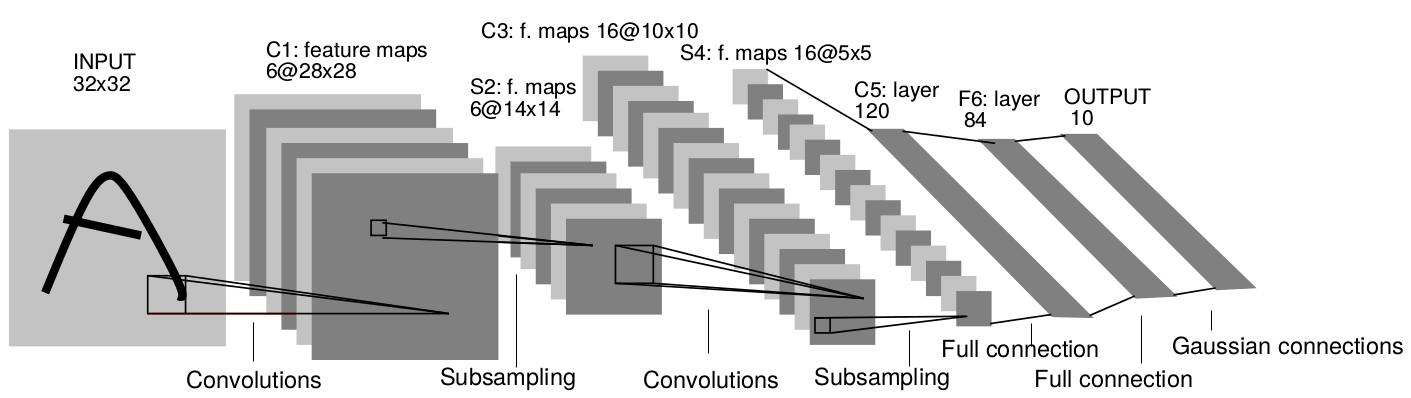
\includegraphics[width=\textwidth]{images/cnns.png}
      \caption[Standard CNN architecture]
              {Standard CNN architecture. Taken
              from~\citep{lecun_gradient-based_1998}}\label{fig:ch2:cnn_generic}
  \end{figure}

\subsection{Fully Connected Layers}\label{sec:ch2:cnn_fullyconnected}
  The convolution, pooling, and activation layers all
  conceptually form part of the \emph{feature extraction} stage of a CNN. One
  or more fully connected layers are usually placed after these layers to form
  the \emph{classifier}. One of the most elegant and indeed most powerful
  features of CNNs is this seamless connection between the \emph{feature
  extraction} and \emph{classifier} sub-networks, allowing the backpropagation
  of gradients through all layers of the entire network.

  The fully connected layers in a CNN are the same as those in a classical
  Neural Network (NN), in that they compute a dot product between their input
  vector and a weight vector:
  \begin{equation}
    z_i = \sum_{j} W_{ij}x_j
  \end{equation}
  The final output of the Fully Connected layer typically has the same number
  of outputs as the number of classes $C$ in the classification problem.

